%%%%%%%%%%%%%%%%%%%%%%%%%%%%%%%%%%%%%%%%%%%%%%%%%%%%%%%%%%%%%%%%
%
% Apuntes de la asignatura Geometría III.
% Doble Grado de Informática y Matemáticas.
% Universidad de Granada.
% Curso 2016/17.
%
%
% Colaboradores:
% Javier Sáez (@fjsaezm)
% Daniel Pozo (@danipozodg)
% Pedro Bonilla (@pedrobn23)
% Guillermo Galindo
% Antonio Coín (@antcc)
% Sofía Almeida (@SofiaAlmeida)
% Miguel Lentisco (@AlfaOmegaX)
%
% Agradecimientos:
% Andrés Herrera (@andreshp) y Mario Román (@M42) por
% las plantillas base.
%
% Sitio original:
% https://github.com/libreim/apuntesDGIIM/
%
% Licencia:
% CC BY-NC-SA 4.0 (https://creativecommons.org/licenses/by-nc-sa/4.0/)
%
%%%%%%%%%%%%%%%%%%%%%%%%%%%%%%%%%%%%%%%%%%%%%%%%%%%%%%%%%%%%%%%


%------------------------------------------------------------------------------
%   ACKNOWLEDGMENTS
%------------------------------------------------------------------------------

%%%%%%%%%%%%%%%%%%%%%%%%%%%%%%%%%%%%%%%%%%%%%%%%%%%%%%%%%%%%%%%%%%%%%%%%
% Plantilla básica de Latex en Español.
%
% Autor: Andrés Herrera Poyatos (https://github.com/andreshp)
%
% Es una plantilla básica para redactar documentos. Utiliza el paquete  fancyhdr para darle un
% estilo moderno pero serio.
%
% La plantilla se encuentra adaptada al español.
%
%%%%%%%%%%%%%%%%%%%%%%%%%%%%%%%%%%%%%%%%%%%%%%%%%%%%%%%%%%%%%%%%%%%%%%%%%

%%%
% Plantilla de Trabajo
% Modificación de una plantilla de Latex de Frits Wenneker para adaptarla
% al castellano y a las necesidades de escribir informática y matemáticas.
%
% Editada por: Mario Román
%
% License:
% CC BY-NC-SA 3.0 (http://creativecommons.org/licenses/by-nc-sa/3.0/)
%%%

%%%%%%%%%%%%%%%%%%%%%%%%%%%%%%%%%%%%%%%%
% Short Sectioned Assignment
% LaTeX Template
% Version 1.0 (5/5/12)
%
% This template has been downloaded from:
% http://www.LaTeXTemplates.com
%
% Original author:
% Frits Wenneker (http://www.howtotex.com)
%
% License:
% CC BY-NC-SA 3.0 (http://creativecommons.org/licenses/by-nc-sa/3.0/)
%
%%%%%%%%%%%%%%%%%%%%%%%%%%%%%%%%%%%%%%%%%


% Tipo de documento y opciones.
\documentclass[11pt, a4paper, titlepage]{article}


%---------------------------------------------------------------------------
%   PAQUETES
%---------------------------------------------------------------------------

% Idioma y codificación para Español.
\usepackage[utf8]{inputenc}
\usepackage[spanish, es-tabla, es-lcroman, es-noquoting]{babel}
\selectlanguage{spanish}
%\usepackage[T1]{fontenc}

% Fuente utilizada.
\usepackage{courier}    % Fuente Courier.
\usepackage{microtype}  % Mejora la letra final de cara al lector.

% Diseño de página.
\usepackage{fancyhdr}   % Utilizado para hacer títulos propios.
\usepackage{lastpage}   % Referencia a la última página.
\usepackage{extramarks} % Marcas extras. Utilizado en pie de página y cabecera.
\usepackage[parfill]{parskip}    % Crea una nueva línea entre párrafos.
\usepackage{geometry}            % Geometría de las páginas.

% Símbolos y matemáticas.
\usepackage{amssymb, amsmath, amsthm, amsfonts, amscd}
\usepackage{upgreek}

% Otros.
\usepackage{enumitem}   % Listas mejoradas.
\usepackage[hidelinks]{hyperref}
\usepackage{pgfplots}
\usepackage{graphicx}   % Gráficos.


%---------------------------------------------------------------------------
%   OPCIONES PERSONALIZADAS
%---------------------------------------------------------------------------

% Redefinir letra griega épsilon.
\let\epsilon\upvarepsilon

% Formato de texto.
\linespread{1.1}            % Espaciado entre líneas.
\setlength\parindent{0pt}   % No indentar el texto por defecto.
\setlist{leftmargin=.5in}   % Indentación para las listas.

% Estilo de página.
\pagestyle{fancy}
\fancyhf{}
\geometry{left=3cm,right=3cm,top=3cm,bottom=3cm,headheight=1cm,headsep=0.5cm}   % Márgenes y cabecera.

% Redefinir entorno de demostración (reducir espacio superior)
\makeatletter
\renewenvironment{proof}[1][\proofname] {\vspace{-15pt}\par\pushQED{\qed}\normalfont\topsep6\p@\@plus6\p@\relax\trivlist\item[\hskip\labelsep\it#1\@addpunct{.}]\ignorespaces}{\popQED\endtrivlist\@endpefalse}
\makeatother

% Aumentar el tamaño del interlineado
\linespread{1.3}
%---------------------------------------------------------------------------
%   COMANDOS PERSONALIZADOS
%---------------------------------------------------------------------------

% Valor absoluto: \abs{}
\providecommand{\abs}[1]{\lvert#1\rvert}

% Fracción grande: \ddfrac{}{}
\newcommand\ddfrac[2]{\frac{\displaystyle #1}{\displaystyle #2}}

% Texto en negrita en modo matemática: \bm{}
\newcommand{\bm}[1]{\boldsymbol{#1}}

% Línea horizontal.
\newcommand{\horrule}[1]{\rule{\linewidth}{#1}}

% Renombrar la R de los reales

\newcommand{\R}{\mathbb{R}}



%---------------------------------------------------------------------------
%   CABECERA Y PIE DE PÁGINA
%---------------------------------------------------------------------------

% Cabecera del documento.
\renewcommand\headrule{
	\begin{minipage}{1\textwidth}
		\hrule width \hsize
	\end{minipage}
}

% Texto de la cabecera.
\lhead{\subject}  % Izquierda.
\chead{}            % Centro.
\rhead{\docauthor}    % Derecha.

% Pie de página del documento.
\renewcommand\footrule{
	\begin{minipage}{1\textwidth}
		\hrule width \hsize
	\end{minipage}\par
}

% Texto del pie de página.
\lfoot{}                                                 % Izquierda
\cfoot{}                                                 % Centro.
\rfoot{Página\ \thepage\ de\ \protect\pageref{LastPage}} % Derecha.


%---------------------------------------------------------------------------
%   ENTORNOS PARA MATEMÁTICAS
%---------------------------------------------------------------------------

% Nuevo estilo para definiciones.
\newtheoremstyle{definition-style} % Nombre del estilo.
{10pt}               % Espacio por encima.
{10pt}               % Espacio por debajo.
{}                   % Fuente del cuerpo.
{}                   % Identación.
{\bf}                % Fuente para la cabecera.
{.}                  % Puntuación tras la cabecera.
{.5em}               % Espacio tras la cabecera.
{\thmname{#1}\thmnumber{ #2}\thmnote{ (#3)}}     % Especificación de la cabecera (actual: nombre en negrita).

% Nuevo estilo para notas.
\newtheoremstyle{remark-style}
{10pt}
{10pt}
{}
{}
{\itshape}
{.}
{.5em}
{}

% Nuevo estilo para teoremas y proposiciones.
\newtheoremstyle{theorem-style}
{10pt}
{10pt}
{\itshape}
{}
{\bf}
{.}
{.5em}
{\thmname{#1}\thmnumber{ #2}\thmnote{ (#3)}}

% Nuevo estilo para ejemplos.
\newtheoremstyle{example-style}
{10pt}
{10pt}
{}
{}
{\scshape}
{:}
{.5em}
{}

% Teoremas, proposiciones y corolarios.
\theoremstyle{theorem-style}
\newtheorem*{nth}{Teorema}
\newtheorem*{nprop}{Proposición}
\newtheorem{ncor}{Corolario}

% Definiciones.
\theoremstyle{definition-style}
\newtheorem*{ndef}{Definición}

% Notas.
\theoremstyle{remark-style}
\newtheorem*{nota}{Nota}

% Ejemplos.
\theoremstyle{example-style}
\newtheorem*{ejemplo}{Ejemplo}

% Listas ordenadas con números romanos (i), (ii), etc.
\newenvironment{nlist}
{\begin{enumerate}
\renewcommand\labelenumi{(\emph{\roman{enumi})}}}
{\end{enumerate}}

% División por casos con llave a la derecha.
\newenvironment{rcases}
  {\left.\begin{aligned}}
  {\end{aligned}\right\rbrace}

%---------------------------------------------------------------------------
%   PÁGINA DE TÍTULO
%---------------------------------------------------------------------------

% Título del documento.
\newcommand{\subject}{Geometría III}

% Autor del documento.
\newcommand{\docauthor}{Doble Grado de Informática y Matemáticas}

% Título
\title{
  \normalfont \normalsize
  \textsc{Universidad de Granada} \\ [25pt]    % Texto por encima.
  \horrule{0.5pt} \\[0.4cm] % Línea horizontal fina.
  \huge \subject\\ % Título.
  \horrule{2pt} \\[0.5cm] % Línea horizontal gruesa.
}

% Autor.
\author{\Large{\docauthor}}

% Fecha.
\date{\vspace{-1.5em} \normalsize Curso 2016/17}


%---------------------------------------------------------------------------
%   COMIENZO DEL DOCUMENTO
%---------------------------------------------------------------------------
\begin{document}

\maketitle  % Título.
\tableofcontents    % Índice
\vfill
\begin{center}
\includegraphics{../Recursos/Plantillas/by-nc-sa.eps}  % Licencia.
\end{center}
\newpage


%----------------------------
%   Introducción.
%----------------------------
\section*{Introducción}
En esta asignatura trataremos de estudiar la geometría afín. Nos centraremos en el plano, el espacio y las figuras que se forman en él.
\newpage

\section{El espacio afín}
\begin{ndef}[Espacio afín]
Dado un conjunto $E$ no vacío diremos que es un espacio afín asociado a un espacio vectorial $V$ si existe la aplicación
$$\varphi: E \times E \rightarrow V$$
$$(a,b) \mapsto \varphi(a,b)$$
tal que se cumplan:
\begin{itemize}
\item Fijado un punto $a$ la aplicación $\varphi_a$ es biyectiva, es decir:
$$\forall a \in E, v \in V, \exists! b \in E:\varphi(a,b)=v$$
\item Se tiene la relación de Charles, es decir:
$$\forall a, b, c \in E \varphi(a,b) + \varphi(b,c) = \varphi(a,c)$$
\end{itemize}
\end{ndef}
\subsection{El plano afín}
Este plano, durante todo el contenido de los apuntes, será el plano $\R^2$. Sabemos que podemos representar un simple punto o un vector dentro de este plano (en este caso, es el plano vectorial). Daremos ahora por sabido todas las propiedades de los vectores.

\begin{tikzpicture}
	\begin{axis}[width=190pt,axis x line=middle, axis y line=center, tick align=outside]
		\addplot+(2,3);
	\end{axis}
\end{tikzpicture}

Lo que haremos es transformar las propiedades de vectores en propiedades de puntos, veamos cómo unir estos dos conceptos.

Sean P y Q dos puntos del plano. Entonces, podemos transformarlos en un vector $\vec{u} = \overrightarrow{PQ} = Q-P$. De la misma forma, analíticamente podemos ver que si tenemos un punto P y le añadimos un vector $\vec{u}$, obtenemos otro punto Q. Damos así por definidas la suma de puntos, vectores y puntos y vectores.

\begin{ndef}[Combinación lineal de vectores]
	Si $u_1,u_2,u_3$ son vectores y $\alpha_1,\alpha_2,\alpha_3$ son escalares, entonces:
	\[
	\alpha_1 u_1+ \alpha_2 u_2 + \alpha_3 u_3
	\]
	es una combinación lineal de vectores.
\end{ndef}

\begin{ndef}[Razón de vectores proporcionales]
	Si $u$ y $v$ son dos vectores proporcionales es decir $u = \lambda v$, entonces se llama a $\lambda$ la razón de esos vectores.
	Si los vectores no son proporcionales no podemos tratar este concepto.
\end{ndef}
Podemos también hacer combinaciones de puntos de la siguiente forma:
\begin{ndef}[Combinaciones baricéntricas de puntos]
	Si $P_1,...,P_n$ son puntos y $\alpha_1,...,\alpha_n \in \R$ pesos de los puntos, que cumplen que $\sum \alpha_i = 1$, entonces una combinación de puntos de la forma:
	\[
	P = \sum_{i=1}^n \alpha_i p_i
	\]
	Es un punto y se le llama combinación baricéntrica de puntos.
\end{ndef}
\begin{proof}
	Lo que haremos, es transformar los puntos en vectores y así la demostración será trivial.

	Restamos primero $P-P_1 = \sum \alpha_i(P_i-P_1)$, así tenemos el vector determinado por $P$ y $P_1$ y una identidad de vectores, de la forma:
	\[
	P-P_1 = \sum_{i=2}^n \alpha_i \overrightarrow{P_1P_i}
	\]

	Y llegamos así a que
	\[
	P = P_1 + \sum_{i=2}^n \alpha_i \overrightarrow{P_1P_i}
	\]
\end{proof}

\begin{ndef}[Combinación convexa]
	Si los pesos $\alpha_i$ asignados a los puntos son todos positivos, llamaremos a su combinación una combinación convexa.
\end{ndef}

\begin{ndef}[Centro de gravedad de unos puntos]
	Si $P_1,...,P_n$ son puntos y $\alpha_1,...,\alpha_n$ son sus pesos, entonces llamamos a
	\[
	\sum_{i=1}^n \alpha_iP_i
	\]
	el centro de gravedad de los puntos.
\end{ndef}

\begin{ndef}[Punto medio]
Sean P y Q dos puntos en el espacio afín. Entonces $m$ es el punto medio entre P y Q si está definido como:
\[
m = \dfrac{1}{2} P + \dfrac{1}{2}Q = \dfrac{1}{2}(P+Q)
\]
Otra forma de hablar de él es: si $u = PQ$, entonces:
\[
m = \dfrac{1}{2}u + P
\]

\end{ndef}

\subsection{Rectas afines}
A partir de ahora, cada vez que mencionemos una recta, estaremos hablando de una recta afín.

\begin{ndef}[Recta vectorial]
	Una recta vectorial es un subespacio vectorial de dimensión 1. Estas están generadas por un vector. De hecho, se notan como $L(v)$ con $v$ un vector.
\end{ndef}

\begin{nprop}
	Si $P$ es un punto y $v$ un vector, entonces la recta afín $r$ viene dada por
	\[
	r = P+L(v) = \{P + \lambda v : \lambda \in \R\}
	\]
	Además, notaremos a $L(v) = \vec{r}$.
\end{nprop}
\begin{ndef}[Variedad de dirección]
	Si $v$ es un vector director, llamaremos variedad de dirección a $L(v) = \vec{r}$.
\end{ndef}

\textbf{Propiedades:}
\begin{itemize}
	\item Si $Q$ es un punto y $Q\in r \implies r = Q +L(v)$
	\item Si $P,Q$ son dos puntos, entonces por ellos pasa una recta y esta es única. Esta recta se nota : $r = P +L(\overrightarrow{PQ})$\\
	\begin{proof}
	Si la recta $r$ pasa por $P$ y $Q$, sea $s$ otra recta que pasa por ellos, entonces:
	\[
	s = P+L(\overrightarrow{PQ}) = r
	\]
\end{proof}
\end{itemize}

\subsubsection{Posición relativa entre rectas}
Según se encuentren en el plano afín, dos rectas $r$ y $s$ pueden ser:
\begin{itemize}
	\item Paralelas, notado $r\parallel s \equiv \vec{r} = \vec{s}$
	\item No paralelas, notado $r\nparallel s \equiv$  sus vectores directores son linealmente independientes $\equiv u$ y $v$ es base.
\end{itemize}

\begin{nth}
	Si $r$, $s$ son dos rectas del plano afín, entonces:
	\begin{nlist}
	\item $r \nparallel s\implies r \cap s = $ un punto
	\item $r \parallel s \implies r = s$ ó $r \cap s =  \emptyset$
\end{nlist}
\begin{proof}
	\begin{nlist}
	\item Si $u,v$ son los vectores directores de $r$ y $s$, entonces con los pares $\{u,v\}$ tenemos que $P+\lambda u = Q + \mu v$ con $\lambda, \mu \in \R$
y si $r = P +L(u)$ y $s=Q+L(v)$, y $\overrightarrow{PQ} = \lambda u - \mu v $ y, por ello, existen únicos $\lambda, \mu$.
\item Sean $u,v$ son los vectores directores de $r$ y $s$. Supongamos que tienen al menos un punto  A en común. Entonces como se podrían escribir estas rectas como $r = A +L(u)$ y $s=A+L(v)$ y además como $r \parallel s \implies L(r)=L(s)$ descubrimos que $r = A +L(u)=A+L(v) = s$.
\end{nlist}
\end{proof}
\end{nth}




\subsection{Triángulos}
Son polígonos que vienen dados por tres puntos no alineados $A,B,C$, que son sus vértices y las tres rectas que los unen.

\begin {ndef}
	Dos o más puntos $A_1, A_2, ... , A_n $ estan alineados $\iff$ existe una recta $r \subset \mathbb{R}^2\ tal\ que\ A_i \in r\ \forall i \in 1,...,n$
\end{ndef}


\begin{nprop}
$A,B,C$ son puntos no alineados  $ \iff \vec{AB},\vec{AC}$ son linealmente independientes.
	\begin {proof}

	\boxed{\Rightarrow}
		Si $\nexists r \subset \mathbb{R}^2\ tal\ que\ A_i \in r\ \forall i \in 1,...,n \Rightarrow \nexists \vec{v}\ tal\ que\ A,B,C \in r = A + L(\vec{v}) \Rightarrow \vec{AB} \neq \alpha \cdot \vec{AC}, \alpha \in \mathbb{R}\ $ porque si no se daría el caso anterior. \\
	\boxed{\Leftarrow} Si A, B, C están en la misma recta, entonces la recta (única) que proporcionan los puntos A y B, y los puntos A y C son la misma, luego $r = A + L(\vec{AB})  = A + L(\vec{AC})$ y entonces $\vec{AB}$ y $\vec{AC}$ serían linealmente dependientes. Como sabemos que $\vec{AB}$ y $\vec{AC}$ no lo son, por lo tanto A, B y C no están alineados.
	\end {proof}

\end{nprop}

% Posibilidad de hacer dibujo de triangulo con los 3 puntos y las 3 rectas



\begin{nth}
	Si consideramos los triángulos $ABC$ y $A_1B_1C_1$ con dos de los lados homólogos paralelos y las razones de los vectores de esos lados son iguales.
	Si las rectas paralelas son: $A\vee C \parallel A_1C_1$ y $A\vee B \parallel A_1B_1$, por lo que las razones son:
	\[
	\frac{\vec{A_1C_1}}{\vec{AC}} = \frac{\vec{A_1B_1}}{\vec{AB}}
	\]
	Entonces, la pareja restante $C\vee B \parallel C_1B_1$ y $\frac{\vec{B_1C_1}}{\vec{BC}} = \frac{\vec{A_1B_1}}{\vec{AB}} = \frac{\vec{A_1C_1}}{\vec{AC}}$\\
	\begin{proof}
	Si los lados son paralelos, entonces los vectores directores son proporcionales.

	Si $w$ (el lado no mencionado del primer triangulo) es $w=-u+v$ y $w_1$(el lado no mencionado del segundo triángulo) es $w_1 = - \lambda u + \lambda v = \lambda (-u+v) = \lambda w$  por lo que tenemos lo que queríamos.
\end{proof}
\end{nth}

\begin{ndef}[Triángulo medio]
	Si $ABC$ es un triángulo y $A'$,$B'$,$C'$ los puntos medios de sus lados, entonces:
	\begin{nlist}
	\item $A'B'C'$ es un triángulo
	\item Los lados homólogos son paralelos y que el factor de proporcionalidad es: $-\dfrac{1}{2}$
\end{nlist}\vspace{0.2cm}
\begin{proof}

	\begin{nlist}
	\item Se hace viendo que si ABC no están alineados, estos 3 tampoco
	\item Tenemos que: $A' = B/2 + C/2$, $B' = A/2+C/2$, $C' = A/2 + B/2$. Tenemos por tanto que: $\vec{A'B'} = B'-A' = \dfrac{1}{2}(A-B) = -\dfrac{1}{2} \vec{AB}$ y por tanto los lados homólogos son paralelos.

Además, el factor es el número obtenido en la conversión, es decir $\dfrac{-1}{2}$.
\end{nlist}
\end{proof}
\end{ndef}

\begin{ndef}[Medianas de un triángulo]
Las medianas de un triángulo $ABC$ son las rectas que unen un vértice con el punto medio del lado opuesto
\end{ndef}
\begin{ndef}[Baricentro de un triángulo]
	El baricentro $G$ de un triángulo que viene dado por:
	\[
	G = \dfrac{1}{3} A +  \dfrac{1}{3} B +  \dfrac{1}{3} C
	\]
\end{ndef}

\begin{nth}
	Si $ABC$ es un triángulo en el plano afín, entonces las medianas son concurrentes. Su punto de corte es el Baricentro. El baricentro triseca el segmento que une un vértice con el punto medio homólogo.


\end{nth}
	\begin{nth}
	Sea $A'$ el punto medio del lado opuesto a A en un triángulo $ABC$. Sea $AvA'$ una de las medianas. Esta es:
	\[
	\{\lambda A + \mu A': \lambda, \mu \in \R \text{ , } \lambda+\mu = 1\}
	\]
	Entonces, sabemos que $G = \dfrac{1}{3} A +  \dfrac{1}{3} B +  \dfrac{1}{3} C$ y veamos que este está en la mediana: Tenemos que ver la ecuación:
	\[
	G = \dfrac{1}{3} A +  \dfrac{1}{3} B +  \dfrac{1}{3} C = \lambda A + \mu A'  \implies \dfrac{1}{3}A + \dfrac{2}{3}(\dfrac{1}{2}B+\dfrac{1}{2}C) = ... = G
	\]

\end{nth}


\subsection{Ecuaciones de una recta}
Hemos visto una recta como un punto $A$ y un vector $\vec{v}$. Es decir, $r \equiv (x_0,y_0) +(x,y) : (x,y) \in L(v) \equiv (x_0+x,y_0+y) $.

También por tanto podemos hacer una recta mediante dos puntos, tomando el vector que forman esos dos puntos y uno de ellos y teniendo la situación anterior.

Las rectas vectoriales en el plano vectorial son siempre de la forma:
\[
\vec{r} \equiv (x,y) \in L : \alpha x + \beta y = 0 \text{  con $\alpha$ o $\beta$ distinto de 0}
\]

Si $r$ es una recta afín, entonces:
\[
r \equiv \alpha x + \beta y = \gamma
\] con $\alpha$ o $\beta$ distintos de $0$ y $\alpha,\beta,\gamma \in \R$

Ahora, si tenemos $r'\equiv \alpha' x + \beta' x = \gamma '$ podemos ver que:
\begin{itemize}
	\item $r \parallel r' \iff (\alpha,\beta), (\alpha',\beta') $ son linealmente dependientes. Es decir, si el determinante que forman es $0$

	\item $r \nparallel r'\iff (\alpha,\beta), (\alpha',\beta') $ no son linealmente dependientes. Es decir, si el determinante que forman no es $0$
\end{itemize}

\subsection{Cuadriláteros}

\begin{ndef}
	$ABCD$ es un cuadrilátero que está formado por 4 puntos consecutivos no alineados 3 a 3. Se llaman lados a los segmentos que unen los vertices consecutivos, y diagonales a los segmentos que unen $A \vee C$ y $B \vee D$.
\end{ndef}

\begin{ndef}[Lado]
	Un lado es una recta que une dos vértices consecutivos. En concreto, los cuadriláteros tienen 4 lados: $A \vee B$, $B \vee C$, $C \vee D$
	y $D \vee A$.
\end{ndef}

\begin{ndef}[Diagonal]
	Una diagonal es una recta que une dos vertices no consecutivos. En concreto, los cuadriláteros tienen 2 diagonales: $A \vee C$ y $B \vee D$.
\end{ndef}

% Revisar
\begin{ndef}[Paralelogramo]
	Un paralelogramo es un cuadrilátero que cumple que todos sus lados opuestos son paralelos. Es decir, sea $ABCD$ un
	paralelogramo entonces $AvB$ es paralelo a $C \vee D$ y $B \vee C$ es paralelo a $D \vee A$. Además los paralelogramos cumplen que:
	- Sea $V_{1} = A \vee B$, $V_{2} = B \vee C$, $V_{3} = C\vee D$, $V_{4} = D \vee A$ entonces:
	\begin{nlist}
		\item $V_{1} - V_{2} - V_{3} + V_{4} = 0$
		\item $V_{3} = \lambda V_{1} con \lambda \neq 0$
		\item $V_{4} = \mu V_{2} con \mu \neq 0$
	\end{nlist}
\end{ndef}


\begin{nprop}
	Sea ABCD un cuadrilátero. Entonces, son equivalentes:
	\begin{nlist}
		\item ABCD es un paralelogramo
		\item $\vec{AB} = \vec{DC}$
		\item Las diagonales del cuadrilátero se cortan en su punto medio.
	\end{nlist}
\end{nprop}
% Falta revisar y 3) => 1)
\begin{proof}\hfill
	\boxed{1) \Rightarrow 2)}
	Solo tenemos que fijarnos en lo que implica ser paralelogramo (ver propiedad arriba):
	$V_{1} - V_{2} - V_{3} + V_{4} = 0 \Leftrightarrow V_{1} - V_{2} = V_{3} - V_{4} $
	Sustituimos $V_{3} = \lambda V_{1}$ y $V_{4} = \mu V_{2}$:
	$V_{1} - V_{2} = \lambda V_{1} - \mu V_{2}$
	Como sabemos que $V_{1} y V_{2}$ unen 3 puntos que no están alineados, entonces sabemos que son linealmente independientes y por
	tanto forman base, por esta razon, cualquier vector se forma como combinación lineal de ellos, con coeficientes únicos.
	Concluyendo por tanto que entonces $\lambda = 1 y \mu = 1$

	\boxed{2) \Rightarrow 3)}
	Tenemos que $B - A = C - D$, pasando los términos:
	$B + D = C + A$
	Y ahora dividiendo todo entre 2:
	$\frac{1}{2}B + \frac{1}{2}D = \frac{1}{2}C + \frac{1}{2}A$
	Con lo cual obtenemos los puntos medios de las diagonales que son iguales.

	\boxed{3) \Rightarrow 1)}
	%Falta completar
\end{proof}

\end{document}
